La librería \emph{mpegparser} provee la funcionalidad necesaria para obtener las secciones de control y los flujos de audio, video y datos
de un TS (Transport Stream). Para esto, cuenta con 3 grupos principales de clases, \hyperlink{classtuner_1_1Provider}{\texttt{Provider}}, \hyperlink{classtuner_1_1demuxer_1_1ts_1_1Demuxer}{\texttt{Demuxer}} y \hyperlink{classtuner_1_1Service}{\texttt{Service}}. 

\texttt{Provider} permite acceder a las distintas secciones de control del TS (PAT, PMT, NIT, etc) y los flujos de datos (Audio, Video y Datos), haciendo uso de distintos filtros.

El grupo de clases correspondientes a \texttt{Demuxer}, permite demultiplexar las secciones de control y los flujos de datos obtenidos a partir de filtros, también permite notificar la ocurrencia de los mismos. 

Finalmente, las clases pertenecientes al grupo Service proveen una abstracción de los servicios de MPEG, permitiendo acceder a los diferentes servicios contenidos en el TS de manera transparente.

\begin{figure}[h!]
	\centering
	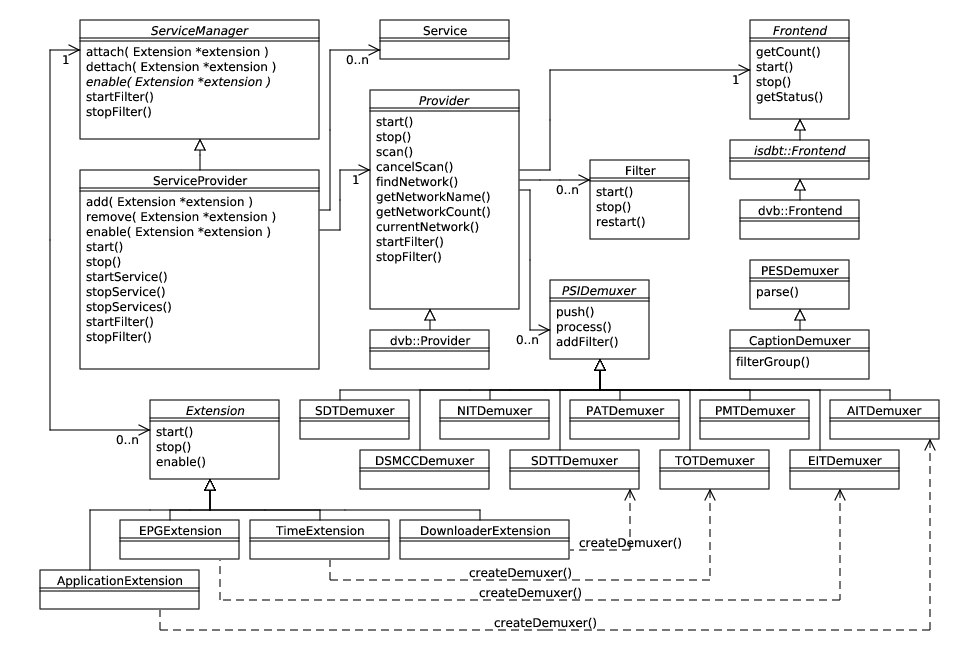
\includegraphics[scale=0.5]{resources/uml-dtv-mpegparser.jpg}
	\caption{Diagrama de las principales clases de la librería \emph{mpegparser}.}
\end{figure}

\FloatBarrier
